\documentclass[10pt,landscape]{article}
\usepackage{multicol}
\usepackage[landscape]{geometry}
\usepackage[procnames]{listings}
\usepackage[parfill]{parskip}
\usepackage{fixltx2e}
\usepackage[T1]{fontenc}
\usepackage{lmodern}
\usepackage{graphicx}

% "define" Scala
\usepackage[T1]{fontenc}  
\usepackage[scaled=0.82]{beramono}  
\usepackage{microtype} 

\sbox0{\small\ttfamily A}
\edef\mybasewidth{\the\wd0 }

\lstdefinelanguage{scala}{
  morekeywords={abstract,case,catch,class,def,%
    do,else,extends,false,final,finally,%
    for,if,implicit,import,match,mixin,%
    new,null,object,override,package,%
    private,protected,requires,return,sealed,%
    super,this,throw,trait,true,try,%
    type,val,var,while,with,yield},
  sensitive=true,
  morecomment=[l]{//},
  morecomment=[n]{/*}{*/},
  morestring=[b]",
  morestring=[b]',
  morestring=[b]"""
}

\usepackage{color}
\definecolor{dkgreen}{rgb}{0,0.6,0}
\definecolor{gray}{rgb}{0.5,0.5,0.5}
\definecolor{mauve}{rgb}{0.58,0,0.82}

% Default settings for code listings
\lstset{frame=tb,
  language=scala,
  aboveskip=3mm,
  belowskip=3mm,
  showstringspaces=false,
  columns=fixed, % basewidth=\mybasewidth,
  basicstyle={\small\ttfamily},
  numbers=none,
  numberstyle=\footnotesize\color{gray},
  % identifierstyle=\color{red},
  keywordstyle=\color{blue},
  commentstyle=\color{dkgreen},
  stringstyle=\color{mauve},
  frame=single,
  breaklines=true,
  breakatwhitespace=true,
  procnamekeys={def, val, var, class, trait, object, extends},
  procnamestyle=\ttfamily\color{red},
  tabsize=2
}

\lstnewenvironment{scala}[1][]
{\lstset{language=scala,#1}}
{}
\lstnewenvironment{cpp}[1][]
{\lstset{language=C++,#1}}
{}
\lstnewenvironment{bash}[1][]
{\lstset{language=bash,#1}}
{}
\lstnewenvironment{verilog}[1][]
{\lstset{language=verilog,#1}}
{}



% Remove section numbering
\setcounter{secnumdepth}{0}

\geometry{top=.75cm,left=.75cm,right=.75cm,bottom=.75cm}


\pagestyle{empty}
\setlength{\parskip}{0cm}

\makeatletter
\renewcommand{\section}{\@startsection{section}{1}{0mm}%
                                {-0.5ex plus 4ex}%
                                {-0.01ex plus .01ex}%x
                                {\normalfont\large\bfseries}}
\renewcommand{\subsection}{\@startsection{subsection}{2}{0mm}%
                                {-0.5ex plus 4ex}%
                                {-0.01ex plus .01ex}%
                                {\normalfont\normalsize\bfseries}}
\renewcommand{\subsubsection}{\@startsection{subsubsection}{3}{0mm}%
                                {-0.01ex plus 0.01ex}%
                                {-0.01ex plus .01ex}%
                                {\normalfont\small\bfseries}}
\makeatother

\begin{document}
\begin{multicols}{3}

\newcommand*\ruleline[1]{\par\noindent\raisebox{.8ex}{\makebox[\linewidth]{\hrulefill\hspace{1ex}\raisebox{-.8ex}{#1}\hspace{1ex}\hrulefill}}}
\renewcommand{\tabcolsep}{.5mm}

\ruleline{\Large{\textbf{Chisel Cheat Sheet}}}
\begin{center}
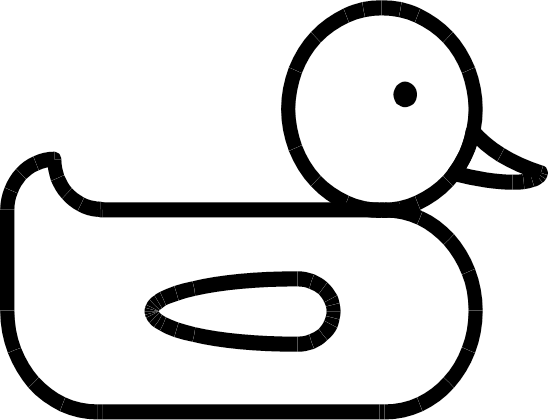
\includegraphics[scale=0.02]{bigduck.png} Version 0.5 (beta): \today
\end{center}

\fbox{ \parbox{0.95\columnwidth} {
\subsection{Notation In This Document}:
\subsubsection{For Functions and Constructors}: \newline
Arguments given as \texttt{kwd:type} (name and type(s)) \newline
Arguments in brackets (\texttt{[...]}) are optional.
\subsubsection{For Operators}: \newline
\texttt{c}, \texttt{x}, \texttt{y} are Chisel \texttt{Data};
\texttt{n}, \texttt{m} are Scala \texttt{Int} \newline
\texttt{w(x)}, \texttt{w(y)} are the widths of \texttt{x}, \texttt{y} (respectively) \newline
\texttt{minVal(x)}, \texttt{maxVal(x)} are the minimum or \newline
\phantom{x} maximum possible values of \texttt{x}
} }

\section{Basic Chisel Constructs } \hrulefill
\subsection{Chisel Wire Operators}: \newline
\begin{tabular}{l l}
\verb$val x = UInt()$ & Allocate \verb$a$ as wire of type \verb$UInt()$ \\
\verb$x := y$ & Assign (connect) wire \verb$y$ to wire \verb$x$ \\
\verb$x <> y$ & Connect \verb$x$ and \verb$y$, wire directionality \\
 & is automatically inferred \\
\end{tabular}

\subsection{When } executes blocks conditionally by \verb$Bool$, \newline
\phantom{x} and is equivalent to Verilog \verb$if$
\begin{scala}
when(condition1) {
  // run if condition1 true and skip rest
} .elsewhen(condition2) {
  // run if condition2 true and skip rest
} .unless(condition3) {
  // run if condition3 false and skip rest
} .otherwise {
  // run if none of the above ran
}
\end{scala}

\subsection{Switch } executes blocks conditionally by data
\begin{scala}
switch(x) {
  is(value1) {
    // run if x === value1
  } is(value2) {
    // run if x === value2
  }
}
\end{scala}

\subsection{Enum } generates value literals for enumerations \newline
\verb$val s1::s2::$ ... \verb$::sn::Nil$ \newline
\verb$    = Enum(nodeType:UInt, n:Int)$ \newline
\begin{tabular}{l l l}
& \verb$s1$, \verb$s2$, ..., \verb$sn$ & will be created as \verb$nodeType$ literals \\
& & with distinct values \\
& \verb$nodeType$ & type of \verb$s1$, \verb$s2$, ..., \verb$sn$ \\
& \verb$n$ & element count \\
\end{tabular}

\subsection{Math Helpers}: \newline
\begin{tabular}{l l}
\verb$log2Up(in:Int): Int$ & $log_2(\texttt{in})$ rounded up \\
\verb$log2Down(in:Int): Int$ & $log_2(\texttt{in})$ rounded down \\
\verb$isPow2(in:Int): Boolean$ & \verb$True$ if \verb$in$ is a power of 2 \\
\end{tabular}

\columnbreak

\section{Basic Data Types } \hrulefill
\subsubsection{Constructors}: \newline
\verb$Bool([x:Boolean])$ \newline
\verb$Bits/UInt/SInt([x:Int/String], [width:Int])$ \newline
\begin{tabular}{l l l}
& \verb$x$ & {\em (optional)} create a literal from Scala type/ \\
& & pased \verb$String$, or declare unassigned if missing \\
& \verb$width$ & {\em (optional)} bit width (inferred if missing) \\
\end{tabular}

\subsubsection{Bits, UInt, SInt Casts}: reinterpret cast except for:\newline
\begin{tabular*}{\columnwidth}{@{\extracolsep{\fill} } l l l}
\verb$UInt$ $\rightarrow$ \verb$SInt$ & Zero-extend to SInt & \\
\end{tabular*}

\subsubsection{Bool Operators}: \newline
\begin{tabular*}{\columnwidth}{@{\extracolsep{\fill} } l l l}
Chisel & Explanation & Width \\
\hline
\hline
\verb$!x$ & Logical NOT & \verb$1$ \\
\verb$x && y$ & Logical AND & \verb$1$ \\
\verb$x || y$ & Logical OR & \verb$1$ \\
\end{tabular*}

\subsubsection{Bits Operators}: \newline
\begin{tabular*}{\columnwidth}{@{\extracolsep{\fill} } l l l}
Chisel & Explanation & Width \\
\hline
\hline
\verb$x(n)$ & Extract bit, \verb$0$ is LSB & \verb$1$ \\
\verb$x(n, m)$ & Extract bitfield & \verb$n - m + 1$ \\
\verb$x << y$ & Dynamic left shift & \verb$w(x) + maxVal(y)$ \\
\verb$x >> y$ & Dynamic right shift & \verb$w(x) - minVal(y)$ \\
\verb$x << n$ & Static left shift & \verb$w(x) + n$ \\
\verb$x >> n$ & Static right shift & \verb$w(x) - n$ \\
\verb$Fill(n, x)$ & Replicate \verb$x$, \verb$n$ times & \verb$n * w(x)$ \\
\verb$Cat(x, y)$ & Concatenate bits & \verb$w(x) + w(y)$ \\
\verb$Mux(c, x, y)$ & If \verb$c$, then \verb$x$; else \verb$y$ & \verb$max(w(x), w(y))$ \\
\hline
\verb$~x$ & Bitwise NOT & \verb$w(x)$ \\
\verb$x & y$ & Bitwise AND & \verb$max(w(x), w(y))$ \\
\verb$x | y$ & Bitwise OR & \verb$max(w(x), w(y))$ \\
\verb$x ^ y$ & Bitwise XOR & \verb$max(w(x), w(y))$ \\
\hline
\verb$x === y$ & Equality{\small\textcolor{red}{(triple equals)}} & \verb$1$ \\
\verb$x != y$ & Inequality & \verb$1$ \\
\hline
\verb$andR(x)$ & AND-reduce & \verb$1$ \\
\verb$orR(x)$ & OR-reduce & \verb$1$ \\
\verb$xorR(x)$ & XOR-reduce & \verb$1$ \\
\end{tabular*}

\subsubsection{UInt, SInt Operators}: (bitwdths given for \verb$UInt$s) \newline
\begin{tabular*}{\columnwidth}{@{\extracolsep{\fill} } l l l}
Chisel & Explanation & Width \\
\hline
\hline
\verb$x + y$ & Addition & \verb$max(w(x), w(y))$ \\
\verb$x - y$ & Subtraction & \verb$max(w(x), w(y))$ \\
\verb$x * y$ & Multiplication & \verb$w(x) + w(y)$ \\
\verb$x / y$ & Division & \verb$w(x)$ \\
\verb$x % y$ & Modulus & \verb$bits(maxVal(y) - 1)$ \\
\hline
\verb$x > y$ & Greater than & \verb$1$ \\
\verb$x >= y$ & Greater than or equal & \verb$1$ \\
\verb$x < y$ & Less than & \verb$1$ \\
\verb$x <= y$ & Less than or equal & \verb$1$ \\
\hline
\verb$x >> y$ & Arithmetic right shift & \verb$w(x) - minVal(y)$ \\
\verb$x >> n$ & Arithmetic right shift & \verb$w(x) - n$ \\
\end{tabular*}

\columnbreak

\section{State Elements } \hrulefill\
\subsection{Registers } retain state until updated \newline
\verb$val my_reg = Reg([outType:Data], [next:Data],$ \newline
\verb$                 [init:Data])$ \newline
\begin{tabular}{l l l}
& \verb$outType$ & {\em (optional)} register type (or inferred) \\
& \verb$next$ & {\em (optional)} update value every clock \\
& \verb$init$ & {\em (optional)} initialization value on reset \\
\end{tabular}
\subsubsection{Updating}: assign to latch new value on next clock: \newline
\verb$my_reg := next_val$ \newline
The last update (lexically, per clock) runs

\subsection{Read-Write Memory } provide addressable memories \newline
\verb$val my_mem = Mem(out:Data, n:Int,$ \newline
\verb$                 seqRead:Boolean)$ \newline
\begin{tabular}{l l l}
& \verb$out$ & memory element type \\
& \verb$n$ & memory depth (elements) \\
& \verb$seqRead$ & only update reads on clock edge \\
\end{tabular}
\subsubsection{Using}: access elements by indexing: \newline
\verb$val readVal = my_mem(addr:UInt/Int)$ \newline
\phantom{x} for synchronous read: assign output to \verb$Reg$ \newline
\verb$mu_mem(addr:UInt/Int) := y$

\section{Modules } \hrulefill
\subsubsection{Defining}: subclass \verb$Module$ with elements, code:
\begin{scala}
class Accum(width:Int) extends Module {
  val io = new Bundle {
    val in = UInt(INPUT,  width)
    val out  = UInt(OUTPUT, width)
  }
  val sum = new Reg(UInt())
  sum := sum + io.in
  io.out := sum
}
\end{scala}
\subsubsection{Usage}: access elements using dot notation: \newline
\phantom{x} (code inside a \verb$Module$ is always running)
\begin{scala}
val my_module = Module(new Accum(32))
my_module.io.in := some_data
val sum := my_module.io.out
\end{scala}

\section{Hardware Generation } \hrulefill
\subsection{Functions } provide block abstractions for code
\subsubsection{Defining}: write Scala functions with Chisel code:
\begin{scala}
def Adder(op_a:UInt, op_b:UInt): UInt = {
  op_a + op_b
}
\end{scala}
\subsubsection{Usage}: hardware is instantiated when called:
\begin{scala}
sum := Adder(UInt(1), some_data)
\end{scala}

\subsection{If/For } can be used to control hardware generation \newline
\phantom{x} and is equivalent to Verilog \verb$generate if$/\verb$for$

\columnbreak

\section{Aggregate Types } \hrulefill
\subsection{Bundle } contains \verb$Data$ types indexed by name
\subsubsection{Defining}: subclass \verb$Bundle$, define components:
\begin{scala}
class MyBundle extends Bundle {
  val a = Bool()
  val b = UInt(width = 32)
}
\end{scala}
\subsubsection{Constructor}: instantiate \verb$Bundle$ subclass: \newline
\verb$val my_bundle = new MyBundle()$
\subsubsection{Inline defining}: define a \verb$Bundle$ type:
\begin{scala}
val my_bundle = new Bundle {
  val a = Bool()
  val b = UInt(width = 32)
}
\end{scala}
\subsubsection{Using}: access elements through dot notation: \newline
\verb$val bundleVal = my_bundle.a$ \newline
\verb$my_bundle.a := Bool(true)$

\subsection{Vec } is an indexable vector of \verb$Data$ types \newline
\verb$val myVec = Vec(elts:Iterable[Data])$ \newline
\begin{tabular}{l l l}
& \verb$elts$ & initial element \verb$Data$ (vector depth inferred) \\
\end{tabular}

\verb$val myVec = Vec.fill(n:Int) {gen:Data}$ \newline
\begin{tabular}{l l l}
& \verb$n$ & vector depth (elements) \\
& \verb$gen$ & initial element \verb$Data$, called once per element \\
\end{tabular}
\subsubsection{Using}: access elements by dynamic or static indexing: \newline
\verb$readVal := myVec(ind:Data/idx:Int)$ \newline
\verb$myVec(ind:Data/idx:Int) := writeVal$
\subsubsection{Functions}: (\verb$T$ is the \verb$Vec$ element's type) \newline
\begin{tabular}{l l l}
& \verb$.forall(p:T=>Bool): Bool$ & AND-reduce \verb$p$ on all elts \\
& \verb$.exists(p:T=>Bool): Bool$ & OR-reduce \verb$p$ on all elts \\
& \verb$.contains(x:T): Bool$ & \verb$True$ if this contains \verb$x$ \\
& \verb$.count(p:T=>Bool): UInt$ & count elts where \verb$p$ is \verb$True$ \\
\end{tabular}
\begin{tabular}{l l l}
& \verb$.indexWhere(p:T=>Bool): UInt$ & \\
& \verb$.lastIndexWhere(p:T=>Bool): UInt$ & \\
& \verb$.onlyIndexWhere(p:T=>Bool): UInt$ & \\
\end{tabular}

\section{Standard Library: Function Blocks } \hrulefill
\subsection{Stateless}: \newline
\verb$PopCount(in:Bits/Seq[Bool]): UInt$ \newline
\phantom{x} Returns number of hot (= 1) bits in \verb$in$

\verb$Reverse(in:UInt): UInt$ \newline
\phantom{x} Reverses the bit order of \verb$in$

\verb$UIntToOH(in:UInt, [width:Int]): Bits$ \newline
\begin{tabular}{l l l}
& \multicolumn{2}{l}{Returns the one-hot encoding of \texttt{in}} \\
& \verb$width$ & {\em(optional, else inferred)} output width \\
\end{tabular}

\verb$OHToUInt(in:Bits/Seq[Bool]): UInt$ \newline
\phantom{x} Returns the \verb$UInt$ representation of one-hot \verb$in$

\columnbreak

\verb$PriorityEncoder(in:Bits/Iterable[Bool]): UInt$ \newline
\phantom{x} Returns the position the least significant \verb$1$ in \verb$in$

\verb$PriorityEncoderOH(in:Bits): UInt$ \newline
\phantom{x} Returns the position of the hot bit in \verb$in$

\verb$Mux1H(in:Iterable[(Data, Bool]): Data$ \newline
\verb$Mux1H(sel:Bits/Iterable[Bool],$ \newline
\verb$      in:Iterable[Data]): Data$ \newline
\verb$PriorityMux(in:Iterable[(Bool, Bits]): Bits$ \newline
\verb$PriorityMux(sel:Bits/Iterable[Bool],$ \newline
\verb$                  in:Iterable[Bits]): Bits$ \newline
\begin{tabular}{l l l}
& \multicolumn{2}{l}{A mux tree with either a one-hot select or multiple} \\
& \multicolumn{2}{l}{\phantom{x} selects (where the first inputs are prioritized)} \\
& \verb$in$ & iterable of combined input and select \verb$(Bool, Bits)$ \\
& & tuples or just mux input \verb$Bits$ \\
& \verb$sel$ & select signals or bitvector, one per input \\
\end{tabular}

\subsection{Stateful}: \newline
\verb$LFSR16([increment:Bool]): UInt$ \newline
\begin{tabular}{l l l}
& \multicolumn{2}{l}{16-bit LFSR (to generate pseudorandom numbers)} \\
& \verb$increment$ & {\em(optional, default True)} shift on next clock \\
\end{tabular}

\verb$ShiftRegister(in:Data, n:Int, [en:Bool]): Data$ \newline
\begin{tabular}{l l l}
& \multicolumn{2}{l}{Shift register, returns \texttt{n}-cycle delayed input \texttt{in}} \\
& \verb$en$ & {\em(optional, default True)} enable \\
\end{tabular}

\section{Standard Library: Interfaces } \hrulefill
\subsection{DecoupledIO } \mbox{is a \texttt{Bundle} with a ready-valid interface}
\subsubsection{Constructor}: \newline
\verb$Decoupled(gen:Data)$ \newline
\begin{tabular}{l l l}
& \verb$gen$ & Chisel \verb$Data$ to wrap ready-valid protocol around \\
\end{tabular}
\subsubsection{Interface}: \newline
\begin{tabular}{c c l l}
& (in) & \verb$.ready$ & ready \verb$Bool$ \\
& (out) & \verb$.valid$ & valid \verb$Bool$ \\
& (out) & \verb$.bits$ & data \\
\end{tabular}

\subsection{ValidIO } is a \verb$Bundle$ with a valid interface
\subsubsection{Constructor}: \newline
\verb$Valid(gen:Data)$ \newline
\begin{tabular}{l l l}
& \verb$gen$ & Chisel \verb$Data$ to wrap valid protocol around \\
\end{tabular}
\subsubsection{Interface}: \newline
\begin{tabular}{c c l l}
& (out) & \verb$.valid$ & valid \verb$Bool$ \\
& (out) & \verb$.bits$ & data \\
\end{tabular}

\subsection{Queue } is a \verb$Module$ providing a hardware queue
\subsubsection{Constructor}: \newline
\verb$Queue(enq:DecoupledIO, entries:Int)$ \newline
\begin{tabular}{l l l}
& \verb$enq$ & \verb$DecoupledIO$ source for the queue \\
& \verb$entries$ & size of queue \\
\end{tabular}
\subsubsection{Interface}: \newline
\begin{tabular}{l l l}
& \verb$.io.enq$ & \verb$DecoupledIO$ source (flipped) \\
& \verb$.io.deq$ & \verb$DecoupledIO$ sink \\
& \verb$.io.count$ & \verb$UInt$ count of elements in the queue \\
\end{tabular}

\columnbreak

\subsection{Pipe } is a \verb$Module$ delaying input data
\subsubsection{Constructor}: \newline
\verb$Pipe(enqValid:Bool, enqBits:Data, [latency:Int])$ \newline
\verb$Pipe(enq:ValidIO, [latency:Int])$ \newline
\begin{tabular}{l l l}
& \verb$enqValid$ & input data, valid component \\
& \verb$enqBits$ & input data, data component \\
& \verb$enq$ & input data as \verb$ValidIO$ \\
& \verb$latency$ & {\em(optional, default 1)} cycles to delay data by \\
\end{tabular}
\subsubsection{Interface}: \newline
\begin{tabular}{l l l}
& \verb$.io.enq$ & \verb$ValidIO$ source (flipped) \\
& \verb$.io.deq$ & \verb$ValidIO$ sink \\
\end{tabular}

\subsection{Arbiters } are \verb$Module$s connecting multiple producers\newline
\phantom{x} to one consumer \newline
\verb$Arbiter$ prioritizes lower producers \newline
\verb$RRArbiter$ runs in round-robin order
\subsubsection{Constructor}: \newline
\verb$Arbiter(gen:Data, n:Int)$ \newline
\begin{tabular}{l l l}
& \verb$gen$ & data type \\
& \verb$n$ & number of producers \\
\end{tabular}
\subsubsection{Interface}: \newline
\begin{tabular}{l l l}
& \verb$.io.in$ & \verb$Vec$ of \verb$DecoupledIO$ inputs (flipped) \\
& \verb$.io.out$ & \verb$DecoupledIO$ output \\
& \verb$.io.chosen$ & \verb$UInt$ input index on \verb$.io.out$, \\
& & does not imply output is valid \\
\end{tabular}

\section{Tester } \hrulefill

\verb$Tester$ is a class with functions for testing \verb$Module$s, connecting and communicating with a simulator: \newline
\begin{tabular*}{\columnwidth}{@{\extracolsep{\fill} } l l}
\verb$reset([n:Int])$ & reset the DUT for \verb$n$ (default 1) clocks \\
\verb$step(n:Int$) & steps the DUT for \verb$n$ clocks \\
\hline \end{tabular*} \begin{tabular*}{\columnwidth}{@{\extracolsep{\fill} } l l l}
\verb$poke(data:Bits, x:BigInt)$ & writes \verb$x$ to wire \verb$data$ \\
\multicolumn{2}{l}{\texttt{poke(data:Aggregate, x:Array[BigInt])}} \\
\multicolumn{2}{l}{\phantom{x} writes values from \texttt{x} to corresponding wires in \texttt{data}} \\
\verb$peek(data:Bits): BigInt$ & reads from wire \verb$data$ \\
\multicolumn{2}{l}{\texttt{peek(data:Aggregate): Array[BigInt]}} \\
\multicolumn{2}{l}{\phantom{x} reads multiple values from source wires in \texttt{data}} \\
\hline \end{tabular*} \begin{tabular*}{\columnwidth}{@{\extracolsep{\fill} } l l l}
\multicolumn{2}{l}{\texttt{expect(good:Boolean, msg:String): Boolean}} \\
\multicolumn{2}{l}{\phantom{x} fails unless \texttt{good} is \texttt{True}, \texttt{msg} should describe the test} \\
\multicolumn{2}{l}{\texttt{expect(data:Bits, target:BigInt): Boolean}} \\
\multicolumn{2}{l}{\phantom{x} fails unless the value in wire \texttt{data} equals \texttt{target}} \\
\end{tabular*}
\subsubsection{Defining}:\newline
Subclass \verb$Tester$ with testing code:
\begin{scala}
class MuxTester(c:Mux) extends Tester(c) {
  for (sel <- 0 until 2) {
    poke(c.io.sel, sel)
    poke(c.io.in0, 0); poke(c.io.in1, 1)
    step(1)
    expect(c.io.out, sel)
  }
}
\end{scala}

\end{multicols}
\end{document}
